%% LyX 2.3.7 created this file.  For more info, see http://www.lyx.org/.
%% Do not edit unless you really know what you are doing.
\documentclass[10pt,english,t,10pt,handout]{beamer}
\usepackage{lmodern}
\usepackage[T1]{fontenc}
\usepackage[utf8]{inputenc}
\setcounter{tocdepth}{1}
\setlength{\parskip}{\smallskipamount}
\setlength{\parindent}{0pt}
\usepackage{babel}
\usepackage{amsbsy}
\usepackage{amstext}
\usepackage{graphicx}
\usepackage[authoryear]{natbib}
\ifx\hypersetup\undefined
  \AtBeginDocument{%
    \hypersetup{unicode=true}
  }
\else
  \hypersetup{unicode=true}
\fi

\makeatletter
%%%%%%%%%%%%%%%%%%%%%%%%%%%%%% Textclass specific LaTeX commands.
% this default might be overridden by plain title style
\newcommand\makebeamertitle{\frame{\maketitle}}%
% (ERT) argument for the TOC
\AtBeginDocument{%
  \let\origtableofcontents=\tableofcontents
  \def\tableofcontents{\@ifnextchar[{\origtableofcontents}{\gobbletableofcontents}}
  \def\gobbletableofcontents#1{\origtableofcontents}
}

%%%%%%%%%%%%%%%%%%%%%%%%%%%%%% User specified LaTeX commands.



\usepackage{tikz}
\usetikzlibrary{positioning}
\usepackage{appendixnumberbeamer}

\usepackage{graphicx}
\usepackage{subfig}

\usetheme[progressbar=frametitle,block=fill,subsectionpage=progressbar]{metropolis}

% margin
\setbeamersize{text margin right=1.5cm}

% colors
\definecolor{DarkRed}{rgb}{0.7,0,0}
%\colorlet{DarkRed}{red!70!black}
\setbeamercolor{normal text}{fg=black}
\setbeamercolor{alerted text}{fg=DarkRed}
\setbeamercolor{progress bar}{fg=DarkRed}
\setbeamercolor{button}{bg=DarkRed}

% width of seperators
\makeatletter
\setlength{\metropolis@titleseparator@linewidth}{1pt}
\setlength{\metropolis@progressonsectionpage@linewidth}{1pt}
\setlength{\metropolis@progressinheadfoot@linewidth}{1pt}
\makeatother

% new alert block
\newlength\origleftmargini
\setlength\origleftmargini\leftmargini
\setbeamertemplate{itemize/enumerate body begin}{\setlength{\leftmargini}{4mm}}
\let\oldalertblock\alertblock
\let\oldendalertblock\endalertblock
\def\alertblock{\begingroup \setbeamertemplate{itemize/enumerate body begin}{\setlength{\leftmargini}{\origleftmargini}} \oldalertblock}
\def\endalertblock{\oldendalertblock \endgroup}
\setbeamertemplate{mini frame}{}
\setbeamertemplate{mini frame in current section}{}
\setbeamertemplate{mini frame in current subsection}{}
\setbeamercolor{section in head/foot}{fg=normal text.bg, bg=structure.fg}
\setbeamercolor{subsection in head/foot}{fg=normal text.bg, bg=structure.fg}

% footer
\makeatletter
\setbeamertemplate{footline}{%
    \begin{beamercolorbox}[colsep=1.5pt]{upper separation line head}
    \end{beamercolorbox}
    \begin{beamercolorbox}{section in head/foot}
      \vskip1pt\insertsectionnavigationhorizontal{\paperwidth}{}{\hskip0pt plus1filll \insertframenumber{} / \inserttotalframenumber \hskip2pt}\vskip3pt% 
    \end{beamercolorbox}%
    \begin{beamercolorbox}[colsep=1.5pt]{lower separation line head}
    \end{beamercolorbox}
}
\makeatother

% toc
\setbeamertemplate{section in toc}{\hspace*{1em}\inserttocsectionnumber.~\inserttocsection\par}
\setbeamertemplate{subsection in toc}{\hspace*{2em}\inserttocsectionnumber.\inserttocsubsectionnumber.~\inserttocsubsection\par}

\makeatother

\begin{document}
\title{4. Transition Path\vspace{-2mm}}
\subtitle{Adv. Macro: Heterogenous Agent Models} 
\author{Jeppe Druedahl, Raphaël Huleux}
\date{2025}

{
\setbeamertemplate{footline}{} 
\begin{frame}

\maketitle



\end{frame}
}

\addtocounter{framenumber}{-1}

\section{Introduction}
\begin{frame}{Introduction}
\vspace{-2mm}
\begin{itemize}
\item <+->\textbf{Last time: }\emph{Stationary equilibrium (steady states)}
\item <+->\textbf{Today:} \emph{Transition path (dynamic responses away
from steady state)}
\item <+->\textbf{Model:} Heterogeneous Agent Neo-Classical (HANC) model
\item <+->\textbf{Code:} 
\begin{enumerate}
\item Based on the \textcolor{DarkRed}{\href{https://github.com/NumEconCopenhagen/GEModelTools}{GEModelTools}}
package
\item Example from \textcolor{DarkRed}{\href{https://github.com/NumEconCopenhagen/GEModelToolsNotebooks}{GEModelToolsNotebooks/HANC}}\\
\end{enumerate}
\item <+->\textbf{Literature: }
\begin{enumerate}
\item Auclert et. al. (2021), >>Using the Sequence-Space Jacobian to Solve
and Estimate Heterogeneous-Agent Models<<
\item Documentation for GEModelTools\\
\item Kirkby (2017)
\end{enumerate}
\end{itemize}
\end{frame}
%
\begin{frame}{Outline}
    \begin{enumerate}
        \item Introduction to transitions with the Ramsey model
        \item Transition path in HA in partial equilibrium
        \item Transition path in HA in general equilibrium: using sequence-space Jacobians
        \item Fake news algorithm: computing SSJ fast
        \item Exercises
        \item First-order approximations of transition paths
    \end{enumerate}
\end{frame}

\begin{frame}{Example I }
\begin{itemize}
\item What do we mean by transition path?
\item Permanent shock to labor supply (think increase in retirement age)
in the macroeconomic model of the Ministry of Finance: \vspace{1cm}\\
 \begin{figure}[H]     \centering     
\includegraphics[width=0.99\linewidth]{figs/MAKRO_ex1.png}     
\end{figure}
\item \vspace{1cm}Note: Permanent shock, so transition path \emph{between}
two different steady states
\end{itemize}
\end{frame}
%
\begin{frame}{Example II}
\begin{itemize}
\item Temporary shock to public spending (i.e. fiscal stimulus during recessions)\\
 \begin{figure}[H]     \centering     
\includegraphics[width=0.7\linewidth]{figs/MAKRO_ex2.png}     
\end{figure}
\item Note: Temporary shock, so model returns to the \emph{same steady state}
\end{itemize}
\end{frame}
%

\section{Ramsey model}
\begin{frame}{Ramsey: Summary}
\begin{itemize}
\item \textbf{Simplified form:}
\begin{align*}
u^{\prime}(C_{t}^{hh}) & =\beta(1+F_{K}(K_{t},1)-\delta)u^{\prime}(C_{t+1}^{hh})\\
K_{t} & =(1-\delta)K_{t-1}+F(K_{t-1},1)-C_{t}^{hh}
\end{align*}
\item \textbf{Production function:} $\Gamma_{t}K_{t}^{\alpha}L_{t}^{1-\alpha}$
\item \textbf{Utility function:} $\frac{\left(C_{t}^{hh}\right)^{1-\sigma}}{1-\sigma}$
\item \textbf{Steady state:
\begin{align*}
K_{ss} & =\left(\frac{\left(\frac{1}{\beta}-1+\delta\right)}{\Gamma_{ss}\alpha}\right)^{\frac{1}{\alpha-1}}\\
C_{ss}^{hh} & =(1-\delta)K_{ss}+\Gamma_{ss}K_{ss}^{\alpha}-K_{ss}
\end{align*}
}
\end{itemize}
\end{frame}
%
\begin{frame}{Ramsey: As an equation system}

\begin{align*}
\left[\begin{array}{c}
r_{t}^{K}-\alpha\Gamma_{t}K_{t-1}^{\alpha-1}L_{t}^{1-\alpha}\\
w_{t}-(1-\alpha)\Gamma_{t}K_{t-1}^{\alpha}L_{t}^{-\alpha}\\
r_{t}-(r_{t}^{K}-\delta)\\
A_{t}-K_{t}\\
A_{t}^{hh}-\left((1+r_{t})A_{t-1}^{hh}+w_{t}L_{t}^{hh}-C_{t}^{hh}\right)\\
C_{t}^{hh,-\sigma}-\beta(1+r_{t+1})C_{t+1}^{hh,-\sigma}\\
A_{t}-A_{t}^{hh}\\
L_{t}-L_{t}^{hh}\\
\forall t\in\{0,1,\dots\},\text{given }K_{-1}
\end{array}\right] & \boldsymbol{=}\boldsymbol{0}
\end{align*}
\textbf{Remember:} Perfect foresight w.r.t aggregate variables\\
\textbf{Unknowns}: $\{r_{t}^{K},w_{t},L_{t},K_{t},r_{t},A_{t},C_{t}^{hh},A_{t}^{hh}\}$
for $\forall t\in\{0,1,\dots\}$
\end{frame}
%
\begin{frame}{Recap: Newton's method I}
\begin{itemize}
\item <+->Before solving the dynamic Ramsey model, consider a simpler example 
\item <+->Want to solve 1 eq. with 1 unknown (x is a scalar):
\[
f\left(x\right)=0
\]
\item <+->\textbf{How to find} x? First-order Taylor approximation around
current guess $x^{i}$:
\[
f\left(x\right)\approx f\left(x^{i}\right)+f'\left(x^{i}\right)\left(x-x^{i}\right)
\]
\item <+->Set $f\left(x\right)=0$ and solve for x to get:
\[
x=x^{i}-\frac{f\left(x^{i}\right)}{f'\left(x^{i}\right)}
\]
\end{itemize}
\end{frame}
%
\begin{frame}{Recap: Newton's method II }
\begin{itemize}
\item <+->Newton's method: Given initial guess $x_{0}$ update guess for
$x$ from $i$ to $i+1$ as:
\[
x^{i+1}=x^{i}-\frac{f\left(x^{i}\right)}{f'\left(x^{i}\right)}
\]

\begin{itemize}
\item until $\left|f\left(x^{i}\right)\right|<\epsilon$
\end{itemize}
\item <+->Can always get $f\left(x^{i}\right)$ by simply evaluating the
function at current estimate. What about derivative $f'\left(x^{i}\right)$?
\item <+->Use numerical approximation:
\[
f'\left(x^{i}\right)\approx\frac{f\left(x^{i}+h\right)-f\left(x^{i}\right)}{h}
\]

\begin{itemize}
\item For small $h$.
\end{itemize}
\item <+->How well does it work?
\begin{itemize}
\item If $f\left(x\right)$ is linear this update solves $f\left(x\right)=0$
in \textbf{1 iteration}
\item If $f\left(x\right)$ is non-linear we typically need more iterations,
but works well if initial guess is within basis of attraction
\end{itemize}
\end{itemize}
\end{frame}
%
\begin{frame}{Recap: Multivariate Newton's method}
\begin{itemize}
\item <+->Generalize to vector-valued, multivariate functions $\left[f_{1}\left(x_{1,}x_{2}\right),f_{2}\left(x_{1,}x_{2}\right)\right]'=\boldsymbol{f}\left(\boldsymbol{x}\right)$
with $\boldsymbol{x}=\left(x_{1,}x_{2}\right)'$ :
\[
\boldsymbol{x}^{i+1}=\boldsymbol{x}^{i}-\boldsymbol{J}\left(\boldsymbol{x}^{i}\right)^{-1}\boldsymbol{f}\left(\boldsymbol{x}^{i}\right)
\]
\item <+->Where $\boldsymbol{J}\left(\boldsymbol{x}^{i}\right)$ is the
\emph{Jacobian }of\emph{ $f\left(\boldsymbol{x}\right)$ }w.r.t $\boldsymbol{x}^{i}$:
\[
\boldsymbol{J}\left(\boldsymbol{x}_{i}\right)=\left[\begin{array}{cc}
\frac{\partial f_{1}}{\partial x_{1}^{i}} & \frac{\partial f_{1}}{\partial x_{2}^{i}}\\
\frac{\partial f_{2}}{\partial x_{1}^{i}} & \frac{\partial f_{2}}{\partial x_{2}^{i}}
\end{array}\right]
\]
\item <+->Can calculate this jacobian in the same way as $f'\left(x\right)$
in previous example, but need to so for every element in \textbf{$\boldsymbol{x}$}
\item <+->\textbf{Go through code}
\end{itemize}
\end{frame}
%
\begin{frame}{Recap: Broyden's method I}
\begin{itemize}
\item <+->Newton's method updates Jacobian $\boldsymbol{J}$ in \textbf{every
iteration}
\item <+->If $\boldsymbol{J}$ is expensive to calculate, this is a serious
bottleneck 
\item <+->Broyden's method solves this issue by only calculating $J$ around
some initial point.
\item <+->Then apply following (linear) update of $f'\left(x^{i+1}\right)$
at every iteration $i$:
\[
f'\left(x^{i+1}\right)=f'\left(x^{i}\right)+\frac{\left[f\left(x^{i+1}\right)-f\left(x^{i}\right)\right]-f'\left(x^{i}\right)\left(x^{i+1}-x^{i}\right)}{x^{i+1}-x^{i}}
\]
\end{itemize}
\end{frame}
%
\begin{frame}{Recap: Broyden's method II}
\begin{enumerate}
\item Guess $\boldsymbol{x}^{0}$ and set $i=0$
\item Calculate the Jacobian around initial point $\boldsymbol{J}_{\boldsymbol{0}}$
\item Calculate $\boldsymbol{f}^{i}=\boldsymbol{f}(\boldsymbol{x}^{i})$.
\item Stop if $\left|\boldsymbol{f}^{i}\right|$ below tolerance $\epsilon$
\item Calculate Jacobian by $\boldsymbol{J}^{i}=\begin{cases}
\boldsymbol{J}_{\boldsymbol{0}} & \text{if }i=0\\
\boldsymbol{J}^{i-1}+\frac{(\boldsymbol{f}^{i}-\boldsymbol{f}^{i-1})-\boldsymbol{J}^{i-1}(\boldsymbol{x}^{i}-\boldsymbol{x}^{i-1})}{\left|\boldsymbol{x}^{i}-\boldsymbol{x}^{i-1}\right|_{2}}\left(\boldsymbol{x}^{i}-\boldsymbol{x}^{i-1}\right)^{\prime} & \text{if }i>0
\end{cases}$
\item Update guess by $\boldsymbol{x}^{i+1}=\boldsymbol{x}^{i}-\left(\boldsymbol{J}^{i}\right)^{-1}\boldsymbol{f}^{i}$
\item Increment $i$ and return to step 3
\end{enumerate}
\begin{itemize}
\item \textbf{Go through code}
\end{itemize}
\end{frame}
%
\begin{frame}{Back to Ramsey}

\begin{align*}
\left[\begin{array}{c}
r_{t}^{K}-\alpha\Gamma_{t}K_{t-1}^{\alpha-1}L_{t}^{1-\alpha}\\
w_{t}-(1-\alpha)\Gamma_{t}K_{t-1}^{\alpha}L_{t}^{-\alpha}\\
r_{t}-(r_{t}^{K}-\delta)\\
A_{t}-K_{t}\\
A_{t}^{hh}-\left((1+r_{t})A_{t-1}^{hh}+w_{t}L_{t}^{hh}-C_{t}^{hh}\right)\\
C_{t}^{hh,-\sigma}-\beta(1+r_{t+1})C_{t+1}^{hh,-\sigma}\\
A_{t}-A_{t}^{hh}\\
L_{t}-L_{t}^{hh}\\
\forall t\in\{0,1,\dots\},\text{given }K_{-1}
\end{array}\right] & \boldsymbol{=}\boldsymbol{0}
\end{align*}

\begin{itemize}
\item <+->2 issues:
\begin{itemize}
\item <+->Many unknowns (8 eqs per period)
\item <+->In fact, infinitely many since time is infinite, $T\rightarrow\infty$
\end{itemize}
\end{itemize}
\end{frame}
%
\begin{frame}{Truncated Ramsey, reduced vector form}

\vspace{-7mm}
\begin{align*}
\boldsymbol{H}\left(\boldsymbol{K},\boldsymbol{L},\boldsymbol{\Gamma},K_{-1}\right) & =\left[\begin{array}{c}
A_{t}-A_{t}^{hh}\\
L_{t}-L_{t}^{hh}\\
\forall t\in\{0,1,\dots,T-1\}
\end{array}\right]=\boldsymbol{0}
\end{align*}
where $\boldsymbol{X}=(X_{0},X_{1},\dots,X_{T-1})$, $A_{-1}^{hh}=K_{-1}$
and{\small{}
\begin{align*}
r_{t}^{K} & =\alpha\Gamma_{t}(K_{t-1}/L_{t})^{\alpha-1}\\
w_{t} & =(1-\alpha)\Gamma_{t}(K_{t-1}/L_{t})^{\alpha}\\
A_{t} & =K_{t}\\
r_{t} & =r_{t}^{K}-\delta\\
C_{t}^{hh} & =\left(\beta(1+r_{t+1})\right)^{-\sigma}C_{t+1}^{hh}\,\text{(backwards)}\\
L_{t}^{hh} & =1\\
A_{t}^{hh} & =(1+r_{t})A_{t-1}^{hh}+w_{t}L_{t}^{hh}-C_{t}^{hh}\,\text{(forwards)}
\end{align*}
}\textbf{Truncation:} $T<\infty$ fine when $\Gamma_{t}=\Gamma_{ss}$
for all $t>\underline{t}$ with $\underline{t}\ll T$
\end{frame}
%
\begin{frame}{Further reduced}

\vspace{-7mm}
\begin{align*}
\boldsymbol{H}\left(\boldsymbol{K},\boldsymbol{\Gamma},K_{-1}\right) & =\left[\boldsymbol{A}-\boldsymbol{A}^{hh}\right]=\boldsymbol{0}
\end{align*}
where $\boldsymbol{X}=(X_{0},X_{1},\dots,X_{T-1})$, $A_{-1}^{hh}=K_{-1}$
and{\small{}
\begin{align*}
L_{t}=L_{t}^{hh} & =1\\
r_{t}^{K} & =\alpha\Gamma_{t}(K_{t-1}/L_{t})^{\alpha-1}\\
w_{t} & =(1-\alpha)\Gamma_{t}(K_{t-1}/L_{t})^{\alpha}\\
A_{t} & =K_{t}\\
r_{t} & =r_{t}^{K}-\delta\\
C_{t}^{hh} & =\left(\beta(1+r_{t+1})\right)^{-\sigma}C_{t+1}^{hh}\,\text{(backwards)}\\
A_{t}^{hh} & =(1+r_{t})A_{t-1}^{hh}+w_{t}L_{t}^{hh}-C_{t}^{hh}\,\text{(forwards)}
\end{align*}
}{\small\par}

for $\forall t\in\{0,1,\dots,T-1\}$
\end{frame}
%
\begin{frame}{Sequence space}
\begin{itemize}
\item <+->Note: We have now written the model in \emph{sequence space}
\begin{itemize}
\item Representing an entire timepath/\emph{sequence} of variables as a
function of timepath\emph{/sequence} of other variables
\end{itemize}
\item <+->Example: Keynesian consumption function $C_{t}=a+bY_{t}$:
\begin{align*}
\left[\begin{array}{cccc}
C_{0} & C_{1} & C_{2} & \ldots\end{array}\right]' & =a+b\left[\begin{array}{cccc}
Y_{0} & Y_{1} & Y_{2} & \ldots\end{array}\right]'\\
\Leftrightarrow\boldsymbol{C} & =a+b\boldsymbol{Y}\\
\Leftrightarrow\boldsymbol{C} & =f\left(\boldsymbol{Y}\right)
\end{align*}
\item <+->Powerfull since it also applies \emph{non-linear}, forward-looking
and backwards-looking eqs:
\begin{align*}
C_{t} & =a+b_{0}Y_{t}+b_{1}\log Y_{t-4}+b_{2}Y_{t+4}^{2}\\
\Leftrightarrow\boldsymbol{C} & =g\left(\boldsymbol{Y}\right)
\end{align*}
\item <+->As long as we have the sequence $\boldsymbol{Y}$ we can calculate
$\boldsymbol{C}$
\begin{itemize}
\item Will leverage this later when working with the HA model 
\end{itemize}
\end{itemize}
\end{frame}
%
\begin{frame}{Solution in sequence space}
\begin{itemize}
\item \textbf{Truncation:} $T=200$ (transition path should have converged
to ss by then)
\item \textbf{Jacobian:} Find $\boldsymbol{H}_{\boldsymbol{K}}$ by \emph{numerical
differentiation}
\[
\boldsymbol{H}_{\boldsymbol{K}}=\left[\begin{array}{ccc}
\frac{\partial(A_{0}-A_{0}^{hh})}{\partial K_{0}} & \frac{\partial(A_{0}-A_{0}^{hh})}{\partial K_{1}} & \cdots\\
\frac{\partial(A_{1}-A_{1}^{hh})}{\partial K_{0}} & \ddots & \ddots\\
\vdots & \ddots & \ddots
\end{array}\right]
\]
\item \textbf{Transition path:} Given $\boldsymbol{\Gamma}$ and $K_{-1}$
solve $\boldsymbol{H}\left(\boldsymbol{K},\boldsymbol{\Gamma},K_{-1}\right)$
with non-linear equation system solver (e.g. broyden)
\item \textbf{Two types of perfect foresight transitions:}
\begin{enumerate}
    \item \textit{Transitory:} both the initial and terminal conditions are the steady-state values 
    \item \textit{Permanent:} the economy moves from one state to another state (the terminal state must be a stationary one)
\end{enumerate}
\item \textbf{Notebook:} \emph{Ramsey.ipynb}

\end{itemize}
\end{frame}
%
\begin{frame}{Example 1: permanent from low capital}

\textbf{Initially away from steady state: $K_{-1}=0.75K_{ss}$}

\textbf{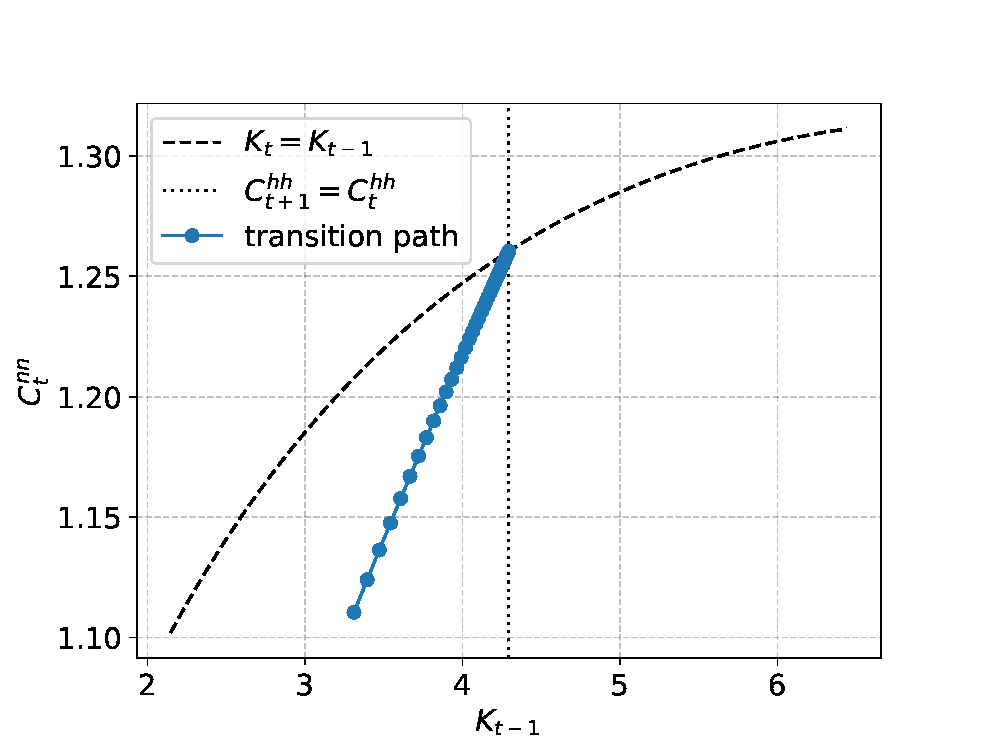
\includegraphics[width=0.8\textwidth]{figs/K_ini_lag}}
\end{frame}
%
\begin{frame}{Example 2: transitory following technology shock}

\textbf{Technology shock: $\Gamma_{t}=0.01\times\Gamma_{ss}\times0.95^{t}$
}(i.e AR(1) with $\rho=0.95$) (exogenous, deterministic)

\textbf{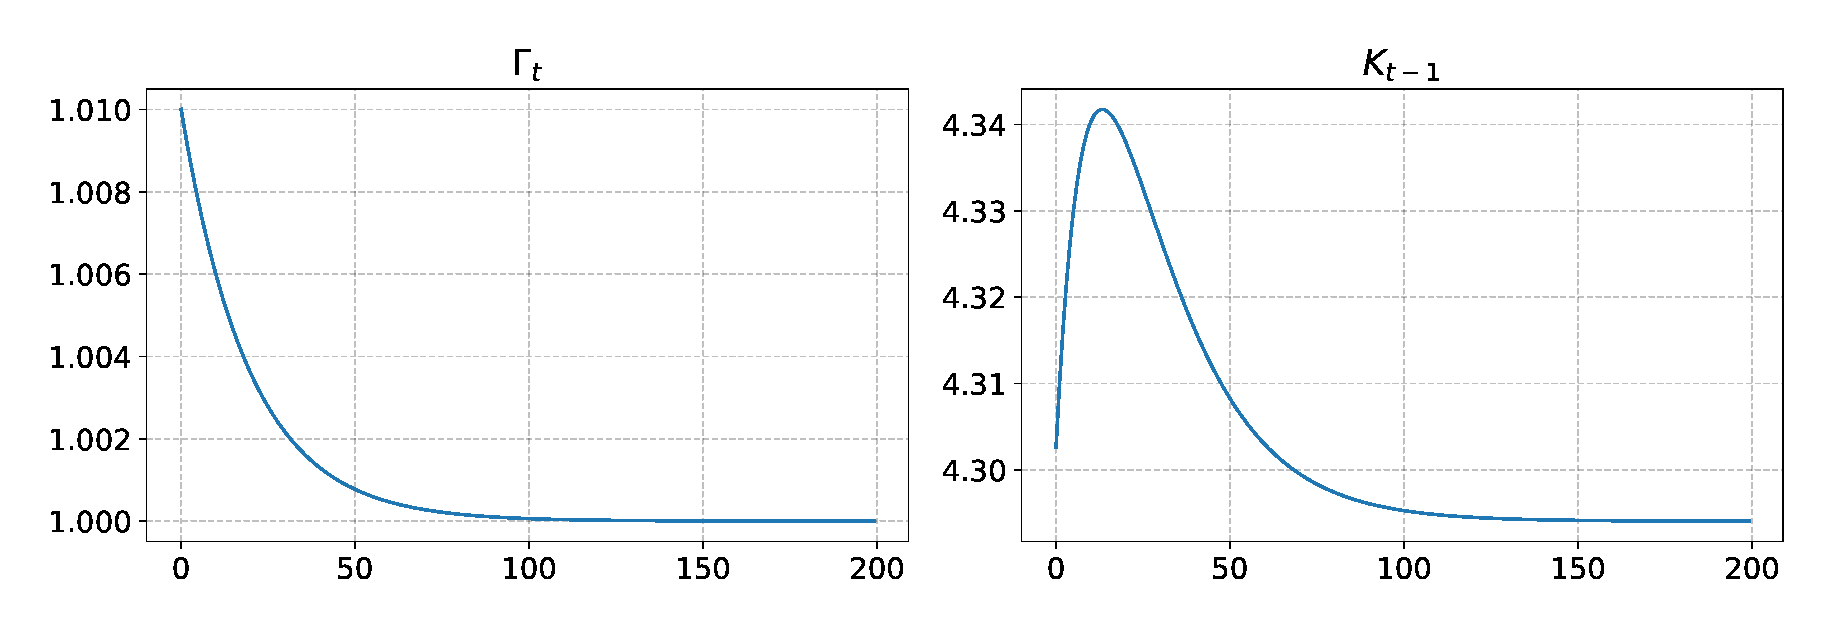
\includegraphics[width=0.95\textwidth]{figs/Gamma_shock}}

\textbf{Terminology:} MIT-shock
\end{frame}
%

\section{Transition path in PE}

\begin{frame}{Household model in a transition}

Recall the household block in the HANC model 
\[\begin{aligned}
v_{0}(z_{it},a_{it-1})&=\max_{\{c_{it}\}_{t=0}^{\infty}}\mathbb{E}_{0}\sum_{t=0}^{\infty}\beta^{t}u(c_{it})\\&\text{s.t.}\\\ell_{it}&=z_{it}\\a_{it}&=(1+r_{t})a_{it-1}+w_{t}\ell_{it}-c_{it}\\\log z_{it+1}&=\rho_{z}\log z_{it}+\psi_{it+1},\,\,\,\psi_{it}\sim\mathcal{N}(\mu_{\psi},\sigma_{\psi}),\,\,\,\mathbb{E}[z_{it}]=1\\a_{it}&\geq0
\end{aligned}\]
Until now, we assume that $r_t=r_{ss}$ and $w_t=w_{ss}$ for all $t$. \pause \\
What if they are time varying-instead? \pause 

\end{frame}


\begin{frame}{Perfect foresight, initial and terminal conditions, }
\textit{Important assumptions: }
\vspace{5mm}
\begin{enumerate}
    \item \textbf{Perfect foresight:} from $t=0$, households know the future path of $\{r_t,w_t\}_{t=0}^\infty$
    \item \textbf{Truncation:} the model converges to a stationary state after $t\geq T$, $T$ large
    \item \textbf{Initial conditions:} we compute the transition from a given distribution $D_0$ that we already know
    \item \textbf{Terminal condition:} we compute a transition towards some stationary state where we know the value function (or its derivative)
\end{enumerate}
\end{frame}

\begin{frame}{Impulse reponses: backward and forward step}

Our goal is to compute a sequence of impulse responses $$A_t^{hh}(\{r_\tau,w_\tau\}_{\tau=0}^T=\int a_t(a,z)dD_t(a,z)\quad \forall t\in(0,T)$$  \pause 
We thus need to obtain a sequence of policy functions $a_t(a,z)$ and distributions $D_t$. \emph{(note the $t$ subscript!)}\pause \\ 
\vspace{5mm}
We will proceed in two steps: \pause 
\begin{enumerate}
    \item \textbf{Backward step}: using the terminal condition on the value function, and going back in time, obtain the policy functions $a_t(a,z)$ and $c_t(a,z)$  \pause 
    \item \textbf{Forward step}: using the initial condition on the distribution, and going forward in time, simulate the distribution over time $D_t(a,z)$
\end{enumerate}

\end{frame}

\begin{frame}{Summing up the transition in PE}
    To solve the household problem, we need three objects:
    \pause 
\begin{enumerate}
    \item An \textbf{exogenous path} of $\{r_t,w_t\}_{t=0}^T$ \pause 
    \item A \textbf{terminal condition} on the value function (or its derivative) $V^a_T(a,z)$ \pause 
    \item An \textbf{initial condition} on the distribution \pause 
\end{enumerate}
We then do a: \pause 
\begin{enumerate}
    \item \textbf{Backward step}, using $V^a_T(a,z)$ as a terminal condition, taking into account $\{r_t,w_t\}_{t=0}^T$ $\to$ this gives us $c_t(a,z)$ and $a_t(a,z)$ \pause 
    \item \textbf{Forward step}, using $D_0(a,z)$ as an initial condition, and $a_t(a,z)$ $\to$ this gives us $D_t(a,z)$ \pause 
\end{enumerate}
We can then obtain the aggregate values of the household as usual by computing
$A_t =\int a_t(a,z)dD_t(a,z).$ This is the \textbf{impulse response}!
\end{frame}

\begin{frame}
\vspace{3cm}
    \begin{center}
        {\huge Let's code!}
    \end{center}
\end{frame}

\section{Transition path in GE}
\begin{frame}{Equation system}

The model can be written as an \textbf{equation system}{\footnotesize{}
\begin{align*}
\left[\begin{array}{c}
r_{t}^{K}-F_{K}(K_{t-1},L_{t})\\
w_{t}-F_{L}(K_{t-1},L_{t})\\
r_{t}-(r_{t}^{K}-\delta)\\
A_{t}-K_{t}\\
\boldsymbol{D}_{t}-\Pi_{z}\underline{\boldsymbol{D}}_{t}\\
\underline{\boldsymbol{D}}_{t+1}-\Lambda_{t}\boldsymbol{D}_{t}\\
A_{t}^{hh}-A_{t}\\
L_{t}^{hh}-L_{t}\\
\forall t\in\{0,1,\dots\},\text{given }\underline{\boldsymbol{D}}_{0}
\end{array}\right] & =\boldsymbol{0}
\end{align*}
}where $\left\{ \Gamma_{t}\right\} _{t\geq0}$ is a given technology
path and $K_{-1}=\int a_{t-1}d\underline{\boldsymbol{D}}_{0}$

\textbf{Remember: }Policies and choice transitions depend on prices
\begin{enumerate}
\item Policy function: $x_{t}^{\ast}=x^{\ast}\left(\left\{ r_{\tau},w_{\tau}\right\} _{\tau\geq t}\right)$
and $X_{t}^{hh}=\sum_{i}x_{it}^{\ast}D_{it}=\boldsymbol{x}_{t}^{\ast\prime}\boldsymbol{D}_{t}$
\item Choice transition: $\Lambda_{t}=\Lambda\left(\left\{ r_{\tau},w_{\tau}\right\} _{\tau\geq t}\right)$
\end{enumerate}
\end{frame}
%
\begin{frame}{Transition path - close to verbal definition}

{\small{}For a given $\boldsymbol{\underline{D}}_{0}$ and a path
$\{\Gamma_{t}\}$\vspace{-1mm}}{\small\par}
\begin{enumerate}
\item {\small{}Quantities $\{K_{t}\}$ and $\{L_{t}\}$,}{\small\par}
\item {\small{}prices $\{r_{t}\}$ and $\{w_{t}\}$,}{\small\par}
\item {\small{}the distributions $\{\boldsymbol{D}_{t}\}$ over $\beta_{i}$,
$z_{t}$ and $a_{t-1}$}{\small\par}
\item {\small{}and the policy functions $\{a_{t}^{\ast}\}$, $\{\ell_{t}^{\ast}\}$
and $\{c_{t}^{\ast}\}$}{\small\par}
\end{enumerate}
{\small{}\vspace{-1mm}are such that in all periods\vspace{-1mm}}{\small\par}
\begin{enumerate}
\item {\small{}Firms maximize profits (prices) }{\small\par}
\item {\small{}Household maximize expected utility (policy functions)}{\small\par}
\item {\small{}$\boldsymbol{D}_{t}$ is implied by simulating the household
problem forwards from $\boldsymbol{\underline{D}}_{0}$}{\small\par}
\item {\small{}Mutual fund balance sheet is satisfied}{\small\par}
\item {\small{}The capital market clears}{\small\par}
\item {\small{}The labor market clears}{\small\par}
\item {\small{}The goods market clears}{\small\par}
\end{enumerate}
\end{frame}
%
\begin{frame}{Reduce size of equation system}
\begin{itemize}
\item In the equation system above we have many \textbf{unknowns} and many
\textbf{equations}
\item <+->Makes finding the solution with Broyden's method since \textbf{Jacobian
is large}
\begin{itemize}
\item With truncation $T$ and $N$ equations/unknowns $\boldsymbol{J}$
has size \textbf{$\left(T\times N,T\times N,\right)$}
\item[$\Rightarrow$] Expensive to calculate 
\end{itemize}
\item <+->We can typically \textbf{exploit model structure }to reduce size
of system 
\begin{itemize}
\item Did this earlier for Ramsey
\item Now more formally 
\end{itemize}
\end{itemize}
\end{frame}
%
\begin{frame}{Truncated, reduced vector form}

\vspace{-7mm}
\begin{align*}
\boldsymbol{H}\left(\boldsymbol{K},\boldsymbol{L},\boldsymbol{\Gamma},\underline{\boldsymbol{D}}_{0}\right) & =\left[\begin{array}{c}
A_{t}^{hh}-A_{t}\\
L_{t}^{hh}-L_{t}\\
\forall t\in\{0,1,\dots,T-1\}
\end{array}\right]=\boldsymbol{0}
\end{align*}
where $\boldsymbol{X}=(X_{0},X_{1},\dots,X_{T-1})$, $K_{-1}=\int a_{t-1}d\underline{\boldsymbol{D}}_{0}$
and{\footnotesize{}
\begin{align*}
r_{t}^{K} & =\alpha\Gamma_{t}(K_{t-1}/L_{t})^{\alpha-1}\\
w_{t} & =(1-\alpha)\Gamma_{t}(K_{t-1}/L_{t})^{\alpha}\\
r_{t} & =r_{t}^{K}-\delta\\
A_{t} & =K_{t}\\
\boldsymbol{D}_{t} & =\Pi_{z}^{\prime}\underline{\boldsymbol{D}}_{t}\\
\underline{\boldsymbol{D}}_{t+1} & =\Lambda_{t}^{\prime}\boldsymbol{D}_{t}\\
A_{t}^{hh} & =\boldsymbol{a}_{t}^{\ast\prime}\boldsymbol{D}_{t}\\
L_{t}^{hh} & =\boldsymbol{\ell}_{t}^{\ast\prime}\boldsymbol{D}_{t}\\
 & \forall t\in\{0,1,\dots,T-1\}
\end{align*}
}\textbf{Truncation:} $T<\infty$ fine when $\Gamma_{t}=\Gamma_{ss}$
for all $t>\underline{t}$ with $\underline{t}\ll T$
\end{frame}
%
\begin{frame}{DAG - Directed Acyclic Graph}
\begin{itemize}
\item \textbf{Orange square:} Shocks (exogenous)
\item \textbf{Blue square:} Unknowns (endogenous)
\item \textbf{Green circles:} Blocks (with variables and targets inside)
\end{itemize}
\centering\includegraphics[width=0.4\textwidth]{figs/DAG} 

\begin{itemize}
\item This DAG implies: Exo. input + guess $\Rightarrow$ Firm block $\Rightarrow$
Mutual fund $\Rightarrow$HHs $\Rightarrow$ Residuals 
\end{itemize}
\end{frame}
%
\begin{frame}{Further reduction}

\vspace{-7mm}
\begin{align*}
\boldsymbol{H}\left(\boldsymbol{K},\boldsymbol{\Gamma},\underline{\boldsymbol{D}}_{0}\right) & =\left[\begin{array}{c}
A_{t}^{hh}(\boldsymbol{w}(\boldsymbol{K}),\boldsymbol{r}(\boldsymbol{K})) - K_t\\
\forall t\in\{0,1,\dots,T-1\}
\end{array}\right]=\boldsymbol{0}
\end{align*}
where $\boldsymbol{X}=(X_{0},X_{1},\dots,X_{T-1})$, $K_{-1}=\int a_{t-1}d\underline{\boldsymbol{D}}_{0}$
and{\footnotesize{}
\begin{align*}
L_{t} & =1\\
r_{t}^{K} & =\alpha\Gamma_{t}(K_{t-1}/L_{t})^{\alpha-1}\\
w_{t} & =(1-\alpha)\Gamma_{t}(K_{t-1}/L_{t})^{\alpha}\\
A_{t} & =K_{t}\\
r_{t} & =r_{t}^{K}-\delta\\
\boldsymbol{D}_{t} & =\Pi_{z}^{\prime}\underline{\boldsymbol{D}}_{t}\\
\underline{\boldsymbol{D}}_{t+1} & =\Lambda_{t}^{\prime}\boldsymbol{D}_{t}\\
A_{t}^{hh} & =\boldsymbol{a}_{t}^{\ast\prime}\boldsymbol{D}_{t}\\
 & \forall t\in\{0,1,\dots,T-1\}
\end{align*}
}\textbf{Truncation:} $T<\infty$ fine when $\Gamma_{t}=\Gamma_{ss}$
for all $t>\underline{t}$ with $\underline{t}\ll T$
\end{frame}
%
\begin{frame}{Solve with Broyden}
\begin{itemize}
\item As with standard Ramsey model from before we have:
\begin{itemize}
\item Equation system with $T$ equations ($\boldsymbol{H}$)
\item And $T$ unknowns ($\boldsymbol{K}$)
\end{itemize}
\item If we can calculate the jacobian of $\boldsymbol{H}$ w.r.t $\boldsymbol{K}$
we can solve with Broyden's method as before
\end{itemize}
\end{frame}
%
\begin{frame}{How to compute Jacobian?}
\begin{itemize}
\item <+->How do we compute the Jacobian of the residuals $\,\boldsymbol{H}$
w.r.t unknowns $\boldsymbol{K}?$
\begin{itemize}
\item Before: Compute Jacobian of entire model using num. diff
\item \textbf{Now}: Use DAG structure + chain rule 
\end{itemize}
\item <+->\emph{Example}. Represent model in block form: \textbf{
\[
\boldsymbol{w},\boldsymbol{r}^{K}=Firm\left(\boldsymbol{K}\right),\quad\boldsymbol{A},\boldsymbol{r}=MutFund\left(\boldsymbol{K},\boldsymbol{r}^{K}\right)
\]
\[
\boldsymbol{A}^{hh}=hh\left(\boldsymbol{r},\boldsymbol{w}\right),\quad\boldsymbol{A}-\boldsymbol{A}^{hh}=\boldsymbol{H}\left(\boldsymbol{A},\boldsymbol{A}^{hh}\right)
\]
}
\item <+-> Collapsing the previous equations, we write the asset-market clearing condition as 
\[\boldsymbol{H}=\boldsymbol{A}^{hh}(\boldsymbol{w}(\boldsymbol{K}),\boldsymbol{r}(\boldsymbol{K})) - \boldsymbol{K}\]
\end{itemize}
\end{frame}
%

\begin{frame}{What is a Jacobian}

Let $\mathcal{J}^{y,x}$ be Jacobian of $y$ w.r.t $x$. Then:
\begin{align*}
\boldsymbol{H}_{\boldsymbol{K}} & = \mathcal{J}^{A^{hh},r}\mathcal{J}^{r,K} +\mathcal{J}^{A^{hh},w}\mathcal{J}^{w,K} - \boldsymbol{I}
\end{align*}

\pause
where 
$$\mathcal{J}^{A^{hh},r}= \left[\begin{matrix}
    \frac{\partial A^{hh}_0}{\partial dr_0} & \frac{\partial A^{hh}_0}{\partial dr_1} & \dots &\frac{\partial A^{hh}_0}{\partial dr_T}\\ 
    \frac{\partial A^{hh}_1}{\partial dr_0} & \frac{\partial A^{hh}_1}{\partial dr_1} & \dots & \frac{\partial A^{hh}_1}{\partial dr_T} \\
    \vdots  & \ddots & \ddots & \vdots \\
    \frac{\partial A^{hh}_T}{\partial dr_0} & \frac{\partial A^{hh}_T}{\partial dr_1} & \dots & \frac{\partial A^{hh}_T}{\partial dr_T}
\end{matrix}\right]$$

\pause
\textbf{Interpretation:} row $t$ of column $s$ gives us the savings change at $t$ in response to a shock on $r$ at $s$.
\pause 
Not just a computational tool, also a lot of economic intuition behind it!
\end{frame}

\begin{frame}{How to compute Jacobian?}    

\begin{itemize}
\item <+->If we have individuals Jacobians, easy to compute $\boldsymbol{H}_{\boldsymbol{K}}$
\begin{itemize}
\item Also very efficient - just matrix mulitiplication \\

\end{itemize}
\item <+->How to get individual Jacobians?
\begin{itemize}
\item Some are easy: For $\mathcal{J}^{w,K},\mathcal{J}^{r,K}$ we just
have to diff. $r_{t}^{K}=\alpha\Gamma_{t}(K_{t-1}/L_{t})^{\alpha-1},w_{t}=(1-\alpha)\Gamma_{t}(K_{t-1}/L_{t})^{\alpha}$
\begin{itemize}
\item Cheap, and can often be vectorized 
\end{itemize}
\item  <+->What about HH Jacobians $\mathcal{J}^{A_{hh},r},\mathcal{J}^{A_{hh},w}$?
\begin{itemize}
    \item Need to compute $T$ impulse reponse!
\end{itemize}
\end{itemize}
\end{itemize}
\end{frame}
%
\begin{frame}{Bottleneck: How do we find the Jacobian?}
\begin{itemize}
\item <+->\textbf{Naive approach: }For each input $i$ into HH block $i\in\left\{ r,w\right\} $
\begin{itemize}
\item For each $s\in\{0,1,...,T-1\}$
\begin{enumerate}
\item Shock input $i$ in period $s$ by small amount $\Delta$
\item Solve household problem backwards along transition path
\item Simulate households forward along transition path
\item Calculate column $s$, row $t$ of jacobian as $\frac{\partial\mathcal{J}_{t}^{A_{hh},i}}{\partial i_{s}}=\frac{A_{t}^{hh}-A_{ss}^{hh}}{\Delta}$
for all $t$
\end{enumerate}
\end{itemize}
\textbf{Bottleneck: }We need $T^{2}$ solution steps and simulation
steps for each input $\left\{ r,w\right\} $!
\item <+->Solution: \textbf{Fake news algorithm} - only need $T$ steps!
(later today)\\
\begin{figure}[H] \centering      
\includegraphics[width=0.3\textwidth]{figs/sequence_space.png}    
\end{figure}
\end{itemize}
\end{frame}

%
\begin{frame}{Summary}
\begin{itemize}
\item Conditional on being able to compute HH jacobian efficiently we can
compute \textbf{transition path }through following steps:
\begin{enumerate}
\item Compute stationary state of model 
\item Formulate transition path as DAG 
\begin{itemize}
\item Reduce number of unknowns and residual equations
\item Not essential, but often good idea 
\end{itemize}
\item Compute Jacobian of residuals $\boldsymbol{H}$ w.r.t unknowns $\boldsymbol{K}$
\item Formulate shock (i.e. TFP increases by 1\% for 4 years)
\item Use Broyden's method to solve for transition path
\end{enumerate}
\end{itemize}
\end{frame}

\begin{frame}
\vspace{3cm}
    \begin{center}
        {\huge Let's code!}
    \end{center}
\end{frame}

\begin{frame}{Reminder}
We are interested in the \textbf{dynamics} of our model \pause 
What we have seen so far:
\begin{enumerate}
    \item How to compute impulse response of the household block in partial equilibrium \pause 
    \begin{enumerate}
        \item Backward step: EGM \pause 
        \item Forward step: histogram method \pause 
    \end{enumerate}
    \item To move to general equilibrium: find the path of an endogenous variable (like $\boldsymbol{K}$) such that markets clear $\boldsymbol{H}(\boldsymbol{\Gamma},\boldsymbol{K})=0$ \pause 
    \item To find $\boldsymbol{K}$, we use Newton's method, which require a \textbf{Sequence Space Jacobian}
\end{enumerate}
\end{frame}

\section{Fake News Algorithm}

\begin{frame}{Fake news algorithm}
\begin{itemize}
\item <+->\textbf{Household block:} 
\begin{align*}
\boldsymbol{Y}^{hh} & =hh(\boldsymbol{X}^{hh})
\end{align*}

\begin{itemize}
\item i.e. $\boldsymbol{Y}^{hh}=C^{hh},A^{hh}$ and $\boldsymbol{X}^{hh}=w,r$
\end{itemize}
\item <+->\textbf{Goal:} Fast computation of
$$\mathcal{J}^{A^{hh},r}= \left[\begin{matrix}
    \frac{\partial A^{hh}_0}{\partial dr_0} & \frac{\partial A^{hh}_0}{\partial dr_1} & \dots &\frac{\partial A^{hh}_0}{\partial dr_T}\\ 
    \frac{\partial A^{hh}_1}{\partial dr_0} & \frac{\partial A^{hh}_1}{\partial dr_1} & \dots & \frac{\partial A^{hh}_1}{\partial dr_T} \\
    \vdots  & \ddots & \ddots & \vdots \\
    \frac{\partial A^{hh}_T}{\partial dr_0} & \frac{\partial A^{hh}_T}{\partial dr_1} & \dots & \frac{\partial A^{hh}_T}{\partial dr_T}
\end{matrix}\right]$$
\item <+->\textbf{Naive approach:} 
\begin{itemize}
\item Shock at time $s=0$, solve + simulate HH block for $T$ periods
\item Repeat until $s=T-1$
\item Requires $T^{2}$ solution and simulation steps 
\end{itemize}
\item <+->\textbf{Next slides: }\emph{Sketch of much faster approach}
\end{itemize}
\end{frame}
%
\begin{frame}{Initial step}
\begin{itemize}
\item Note that aggregate is (matrix) product of individual policy function
$\boldsymbol{y}_{t}$ and distribution $\boldsymbol{D}_{t}$. 
\item Linearize (first-order Taylor) around ss:
\begin{align*}
\boldsymbol{Y}^{hh} & =\left(\boldsymbol{y}_{t}'\right)\boldsymbol{D}_{t}\\
\Rightarrow\frac{d\boldsymbol{Y}^{hh}}{d\boldsymbol{X}^{hh}} & =\left(\frac{d\boldsymbol{y}_{t}}{d\boldsymbol{X}^{hh}}'\right)\boldsymbol{D}_{ss}+\left(\boldsymbol{y}_{ss}'\right)\frac{d\boldsymbol{D}_{t}}{d\boldsymbol{X}^{hh}}
\end{align*}
\item What can we say about policy function term $d\boldsymbol{y}_{t}$?
\end{itemize}
\end{frame}
%
\begin{frame}{Pertubation of policy function}
\begin{itemize}
\item <+->The heart of the fake news algorithm is a central insight that
allow us to compute $d\boldsymbol{y}_{t}/d\boldsymbol{X}^{hh}$ efficiently
\item <+->Let $\boldsymbol{y}_{t}^{s}$ be policy function at time $t$
following a shock in period $s$. Then:
\[
\boldsymbol{y}_{t}^{s}=\begin{cases}
\boldsymbol{y}_{t+j}^{s+j} & t\leq s \\ 
\boldsymbol{y}_{ss} & t>s\\
\end{cases}
\]
\item <+->\textbf{Verbally}: The response of the policy function $\boldsymbol{y}$
at time $t$ to a shock at $s$ is the as the response at time $t+j$
to a shock at $s+j$
\begin{itemize}
\item Policy function \textbf{does not depend on the absolute time of shock}
only the relative distance between >>today<< and the shock, $s-t$.
\end{itemize}
\item <+->\textbf{Implication}: We need to only do a single backwards iteration
to a shock at $s=T-1$. 
\begin{itemize}
\item Can then construct change in policy function $d\boldsymbol{y}_{t}^{s}/d\boldsymbol{X}^{hh}$
for different $s$ by shifting policy function around 
\end{itemize}
\end{itemize}
\end{frame}
%
\begin{frame}{Numerical illustration}

Graphically. Response of $c_{t}$ to income shock at $s=3,5$\\
\begin{figure}[H]  
\centering 
\includegraphics[width=0.6\linewidth]{figs/irf_fakenews1.pdf} 
\end{figure}
\begin{figure}[H]  
\includegraphics[width=0.6\linewidth]{figs/irf_fakenews2.pdf} 
\end{figure}

\end{frame}
%
\begin{frame}{Implementation}
Let's say you want to compute $\frac{d\boldsymbol{A}^{hh}}{d\boldsymbol{w}}$  \pause \\ 
\vspace{5mm}
\underline{Algorithm:}
\begin{enumerate}
    \item Compute the impulse response policy functions to a shock on $w$ at $s=T$ $\to$ obtain a vector of policy functions $\boldsymbol{a}'_t(a,z)$ \pause 
    \item Reconstruct the Jacobian: for all $s\in(0,T)$ \pause 
    \begin{enumerate}
        \item Let \[
\boldsymbol{a}_{t}(a,z)=\begin{cases}
\boldsymbol{a}_{t+j}(a,z) & t\leq s \\
\boldsymbol{a}_{ss}(a,z) & t>s\\
\end{cases}
\] \pause 
        \item Using this reconstructing policy vector, do the forward step  \pause 
        \item Aggregate as usual using $\boldsymbol{A}_t=\int \boldsymbol{a}_t(a,z)dD_t(a,z)$ \pause 
        \item Fill up the column $s$ of the Jacobian as $(\boldsymbol{A}_t-\boldsymbol{A}_{ss})/h$ \pause 
    \end{enumerate}
\end{enumerate}
\end{frame}


\begin{frame}
\vspace{3cm}
    \begin{center}
        {\huge Let's code!}
    \end{center}
\end{frame}


\begin{frame}{Fake news algorithm - summary}
\begin{itemize}
\item <+->Auclert et. al (2021) introduce an efficient algorithm to compute
aggregate jacobians for models with heterogeneous agents 
\begin{itemize}
\item Can compute the linearized response of aggregate consumption, savings
w.r.t aggregate variables such as wages, interest rates \textbf{fast}
\end{itemize}
\item <+->Central insight: Exploit structure of dynamic programming problems
+ histogram method 
\item <+->Why did we need this? 
\begin{itemize}
\item Allows us to compute Jacobian of aggregate model by >>chaining<<
together individual jacobians along DAG
\item Can then use Quasi-Newton methods to solve dynamic GE model!
\end{itemize}
\item <+->GEModeltools does all of this >>under the hood<< when you compute
HH Jacobians
\begin{itemize}
\item You just tell GEModeltools the inputs and outputs of the household
block 
\item Entire algorithm is automated 
\end{itemize}
\end{itemize}
\end{frame}

\section{Linear transitions and aggregate uncertainty}

\begin{frame}{Reminder of model class}

\begin{itemize}
    \item <+-> Unknowns: $\boldsymbol{U}$ 
    \item <+-> Shock: $\boldsymbol{Z}$
    \item <+-> Additional variables: $\boldsymbol{X}$
    \item <+-> Target equation system: $$H(\boldsymbol{U},\boldsymbol{Z})=0$$
    \item <+-> In deterministic, perfect foresigh model (MIT shocks), solve $H(\boldsymbol{U},\boldsymbol{Z})=0$ by 
\begin{enumerate}
    \item Calculating the Jacobian of $H$ w.r.t $\boldsymbol{U}$ around s.s.
    \item Use Newton's method to find non-linear transition given $\boldsymbol{Z}$
\end{enumerate}
$\Rightarrow$ But we have abstracted from real aggregate uncertainty 
\end{itemize}
\end{frame}

\begin{frame}{Aggregate uncertainty}
\begin{itemize}
\item <+->In business cycle model common to have \emph{aggregate uncertainty}
\item <+->I.e. underlying shocks (TFP, demand etc) $x$ follow stochastic
process with dist, $f$, $x_{t}\sim f$
\item <+->This implies that all variables which are functions of $x$ are
also random. 
\begin{itemize}
\item {\small If TFP is random $\Rightarrow$ wages, interest rates, labor
demand etc. are }{\small\textbf{random }}{\small until observed }{\small\par}
\end{itemize}
\item <+->Implies that we need to compute expectation in Euler, NKPC and
other forward looking equations:
\[
u'\left(C_{t}\right)=\beta\mathbb{E}_{t}\left[R_{t+1}\left(x_{t+1}\right)u'\left(C_{t}\left(x_{t+1}\right)\right)\right]
\]
\item <+->Remember: So far in the course we have generally assumed \textbf{perfect
foresight} w.r.t aggregate variables ($w,r$) so no expectation
\begin{itemize}
\item {\small\vspace{-0.5mm}Implies that aggregate shocks are not random
process, but rather }{\small\emph{MIT shocks}}{\small\par}
\item <+->Interpretation of MIT shocks generally hard to reconcile with
business cycles
\end{itemize}
\end{itemize}
\end{frame}

\begin{frame}{Stochastic vs deterministic models}
\begin{itemize}
\item <+->To see how the \textbf{stochastic} model and deterministic model
are related consider the Euler with random $x$: 
\[
u'\left(C_{t}\right)=R\beta\mathbb{E}_{t}\left[u'\left(C_{t}\left(x_{t+1}\right)\right)\right]
\]
\item <+->First-order Taylor approx. around deterministic ss (use $R\beta=1$):
\[
du'\left(C_{t}\right)\approx u''\left(C_{ss}\right)\cdot C'\left(x_{ss}\right)\cdot d\mathbb{E}_{t}x_{t+1}
\]
\item <+->Assume $x_{t}=\rho^{x}x_{t-1}+\epsilon_{t}^{x}$ with $\mathbb{E}\epsilon_{t}^{x}=0$.
Period 0 solution in deterministic/perfect foresight model:
\[
du'\left(C_{0}\right)\approx u''\left(C_{ss}\right)\cdot C'\left(x_{ss}\right)\cdot\rho^{x}d\epsilon_{0}^{x}
\]
\item <+->Stochastic model we use:
\begin{align*}
d\mathbb{E}_{0}x_{1} & =d\mathbb{E}_{0}\left(\rho^{x}x_{0}+\epsilon_{1}^{x}\right)\\
 & =\rho^{x}d\mathbb{E}_{0}x_{0}=\rho^{x}d\epsilon_{0}^{x}=dx_{1}
\end{align*}
\item <+->\vspace{-2mm}Same result! Aggregate uncertainty \textbf{does
not matter to first-order }when linearizing w.r.t aggregate shock
\end{itemize}
\end{frame}


\begin{frame}{Linearized IRFs}
\begin{itemize}

\item Solve for IRfs for unknowns using first-order approximation $$H(\boldsymbol{U},\boldsymbol{Z})=0\Rightarrow H_U d\boldsymbol{U}+ H_{\boldsymbol{Z}} d\boldsymbol{Z}=0\Leftrightarrow d\boldsymbol{U}=\underbrace{-H_U^{-1}H_z }_{=G_U}d\boldsymbol{Z}$$
\item We can find $H_U$ and $H_Z$ as before using fake-news 
\item Limitations:
\begin{itemize}
    \item Imprecise for large shocks
    \item Imprecise in models with aggregate non-linearities
    \item No real aggregate uncertainty (precautionary savings w.r.t. aggregate shocks, etc)
\end{itemize}
\end{itemize}

\end{frame}

\begin{frame}{Linearized IRFs: example from HANC}
You want to compute an IRF facing a TFP shock in HANC. \pause  \\
Recall that
$$H(\boldsymbol{K}, \boldsymbol{\Gamma})=\boldsymbol{A}(\boldsymbol{r}(\boldsymbol{K},\boldsymbol{\Gamma}),\boldsymbol{w}(\boldsymbol{K},\boldsymbol{\Gamma}))-\boldsymbol{K}$$ \pause 
The derivative with respect to $\boldsymbol{K}$ is 
$$
H_{\boldsymbol{K}} = \mathcal{J}^{A^{hh},r}\mathcal{J}^{r,K} +\mathcal{J}^{A^{hh},w}\mathcal{J}^{w,K} - \boldsymbol{I}
$$ \pause 
The derivative with respect to $\boldsymbol{\Gamma}$ is
$$
H_{\boldsymbol{\Gamma}} = \mathcal{J}^{A^{hh},r}\mathcal{J}^{r,\Gamma} +\mathcal{J}^{A^{hh},w}\mathcal{J}^{w,\Gamma} 
$$ \pause 
Write a first-order approximation
$$H_{\boldsymbol{K}} d\boldsymbol{K}+H_{\boldsymbol{\Gamma}}d\boldsymbol{\Gamma}=0 \Leftrightarrow d\boldsymbol{K}= - H_{\boldsymbol{K}} ^{-1}H_{\boldsymbol{\Gamma}}d\boldsymbol{\Gamma}$$ \pause 
This gives us the endogenous response $d\boldsymbol{K}$ for any shock $d\boldsymbol{\Gamma}$ by simply computing the product of two matrices!
    
\end{frame}



\begin{frame}{Simulating a time-series using the linearized solution}
\vspace{-2mm}
We can also simulate the economy following a sequence of shocks: \pause 
\begin{itemize}
\item <+->\textbf{Shocks: }Write the shocks as an $MA(\infty)$ with coefficients
$d\boldsymbol{Z}_{s}$ for $s\in\{0,1,\dots\}$ driven by the innovation
$\boldsymbol{\epsilon}_{t}$. 
\begin{itemize}
\item EX: If shock $\boldsymbol{Z}$ follows an AR(1) then $d\boldsymbol{Z}_{s}=\rho^{s-t}\boldsymbol{\epsilon}_{t-s}$
\end{itemize}
\item <+->\textbf{Linearized simulation:}
\begin{enumerate}
\item <+->Draw time series of innovations, $\tilde{\boldsymbol{\epsilon}}_{t}$
\item <+->Calculate the time series of shocks as $d\tilde{\boldsymbol{Z}}_{t}=\sum_{s=0}^{T-1}d\boldsymbol{Z}_{s}\tilde{\boldsymbol{\epsilon}}_{t-s}$

Note: $d\boldsymbol{Z}_{s}\tilde{\boldsymbol{\epsilon}}_{t-s}=$ effect
of shock $s$ periods ago today 
\item <+->Calculate the time series of other aggregate variables as 
\[
d\tilde{\boldsymbol{X}}_{t}=\sum_{s=0}^{T-1}d\boldsymbol{X}_{s}\tilde{\boldsymbol{\epsilon}}_{t-s}
\]
where $d\boldsymbol{X}_{s}$ is the IRF to a \emph{unit-shock} after
$s$ periods (just needs jacobian of $\boldsymbol{X}$ w.r.t shocks
$\boldsymbol{Z}$)
\end{enumerate}
\item <+->\textbf{Intuition:} Sum of first order effects from all previous
shocks
\end{itemize}
\end{frame}

\begin{frame}
\vspace{3cm}
    \begin{center}
        {\huge Let's code!}
    \end{center}
\end{frame}

\begin{frame}{When does aggregate uncertainty matter?}
\begin{itemize}
\item <+->\textbf{Insight: }\emph{The IRF from an MIT shock is }\emph{\underline{equivalent}}\emph{
to the IRF in a model with aggregate risk, which is linearized in
the aggregate variables} (Boppart et. al., 2018)
\item <+->What about \textbf{high order}?
\item <+->Approximate Euler to \textbf{second} order:
\begin{align*}
du'\left(C_{t}\right)\approx & u''\left(C_{ss}\right)\cdot C'\left(x_{ss}\right)\cdot d\mathbb{E}_{t}x_{t+1}+\frac{1}{2}u'''\left(C_{ss}\right)C''\left(x_{ss}\right)\cdot\mathbb{E}_{t}\left(x_{t+1}-x_{ss}\right)^{2}\\
 & u''\left(C_{ss}\right)\cdot C'\left(x_{ss}\right)\cdot d\mathbb{E}_{t}x_{t+1}+\frac{1}{2}u'''\left(C_{ss}\right)C''\left(x_{ss}\right)\cdot\sigma_{x,t}^{2}
\end{align*}
\item <+->In deterministic model $\sigma_{x,t}^{2}=0$ - not true in stochastic
model!
\begin{itemize}
\item Models deviate once we go beyond 1st order approximation (linearization)
\end{itemize}
\item <+->Still extremely usefull though - we may solve deterministic models
to first-order and interpret as models with aggregate uncertainty
\begin{itemize}
\item How do we linearize models numerically?
\end{itemize}
\end{itemize}
\end{frame}

\begin{frame}{Calculating moments - variance}
\begin{itemize}
\item <+->Implications of prior slide:
\begin{itemize}
\item Very easy to calculate business cycle moments 
\end{itemize}
\item <+->Steps (variance of $C$) (1 shock):
\begin{enumerate}
\item Formulate shock to e.g. public spending, $\left\{ dG_{t}\right\} _{t=0}^{T}=d\boldsymbol{G}$
(could be an AR(1))
\item Linearize and solve model to get IRF of $\left\{ dC_{t}\right\} _{t=0}^{T}=d\boldsymbol{C}$
w.r.t $\left\{ dG_{t}\right\} $
\item Calculate variance $\text{var}(dC_{t})=\sum_{s=0}^{T-1}\left(dC_{s}\right)^{2}$
\end{enumerate}
\item <+->Same principle with more shocks 
\end{itemize}
\end{frame}
%
\begin{frame}{Calculating moments - covariance}
\begin{itemize}
\item <+->\textbf{Covariances:}\vspace{-3mm}
\begin{align*}
\text{cov}(dC_{t},dY_{t+k}) & =\sum_{i\in\mathcal{Z}}\sigma_{i}^{2}\sum_{s=0}^{T-1-k}dC_{s}^{i}dY_{s+k}^{i}
\end{align*}
\item <+->\vspace{-2mm}\textbf{Covariance decomposition:}
\[
\frac{\text{contribution from one shock}}{\text{contributions from all shocks}}=\frac{\sigma_{j}^{2}\sum_{s=0}^{T-1-k}dC_{s}^{j}dY_{s+k}^{j}}{\sum_{i\in\mathcal{Z}}\sigma_{i}^{2}\sum_{s=0}^{T-1-k}dC_{s}^{i}dY_{s+k}^{i}}
\]
 
\end{itemize}
\end{frame}



\begin{frame}{Solving HA model with aggregate risk (advanced)}
\begin{itemize}
\item <+->To solve models with aggregate risk we need to write them in
\emph{state-space} form instead of \emph{sequence-space}
\begin{itemize}
\item Think of HA household problem - that is always in state-space form
\item Endogenous variables $c_{t},a_{t}$ as function of current states
$a_{t-1},z_{t}$
\end{itemize}
\item <+->\textbf{Aggregate stochastic variables: $\boldsymbol{Z}$ }follow
some known process with innovations $\boldsymbol{\epsilon}$. \emph{State
space form}: RHS is what is known today {\small
\[
\left[\begin{array}{c}
\boldsymbol{U}_{t}\\
\boldsymbol{Z}_{t}
\end{array}\right]=\mathcal{M}\left(\left[\begin{array}{c}
\boldsymbol{U}_{t-1}\\
\boldsymbol{Z}_{t-1}
\end{array}\right],\boldsymbol{\epsilon}_{t}\right)
\]
}{\small\par}

$\neq$ perfect foresight wrt. future agg. variables in \emph{sequence-space}
\item <+->In standard NK model: no backward looking eqs. so number of state
variables = Number of shocks 
\end{itemize}
\end{frame}
%
\begin{frame}{Example: Krussel-Smith}
\begin{itemize}
\item <+->What if we add heterogeneous agents? Canonical example: The Krussel-Smith
model (1998) 
\begin{itemize}
\item HANC with aggregate uncertainty (TFP shocks)
\end{itemize}
\item <+->\textbf{Recursive formulation of household problem:}
\begin{align*}
v(\boldsymbol{D}_{t},\Gamma_{t},z_{it},a_{it-1}) & =\max_{a_{it},c_{it}}u(c_{it})+\beta\mathbb{E}_{t}\left[v(\boldsymbol{D}_{t+1},\Gamma_{t+1},z_{it+1},a_{it})\right]\\
 & \text{s.t.}\\
K_{t-1} & =\int a_{it-1}d\boldsymbol{D}_{t}\\
r_{t} & =\alpha\Gamma_{t}K_{t-1}^{\alpha-1}-\delta\\
w_{t} & =(1-\alpha)\Gamma_{t}K_{t-1}^{\alpha}\\
a_{it}+c_{it} & =(1+r_{t})a_{it-1}+w_{t}z_{it}\\
\log z_{it+1} & =\rho_{z}\log z_{it}+\psi_{it+1},\,\,\,\psi_{it}\sim\mathcal{N}(\mu_{\psi},\sigma_{\psi}),\,\,\,\mathbb{E}[z_{it}]=1\\
a_{it} & \geq0,
\end{align*}
\item <+-> \vspace{-2mm}$\boldsymbol{D}_{t}$ is a state variable $\Rightarrow$
Massive state space
\end{itemize}
\end{frame}
%
\begin{frame}{Comparisons}
\begin{itemize}
\item \textbf{State-space approach with linearization}: Ahn et al. (2018);
{\color{DarkRed}\href{https://github.com/BASEforHANK}{Bayer and Luetticke (2020)}};
Bhandari et al. (2023); Bilal (2023)

\underline{Con}: 
\begin{enumerate}
\item Harder to implement
\item Valuable to be able to interpret Jacobians
\end{enumerate}
\underline{Pro}\textbf{:} 
\begin{enumerate}
\item Easier path to 2nd and higher order approximations
\end{enumerate}
\item \textbf{Global solution:} The distribution of households is a state
variable for each household $\Rightarrow$ \emph{explosion in complexity}
\begin{enumerate}
\item \underline{Original}: Krusell and Smith (1997, 1998); Algan et al. (2014);
\item \underline{Deep learning}: Fernández-Villaverde et al. (2021); Maliar
et al. (2021); Han et al. (2021); Kase et al. (2022); Azinovic et
al. (2022); Gu et al. (2023); Chen et al. (2023)
\end{enumerate}
\item \textbf{Discrete aggregate risk:} Lin and Peruffo (2023)
\end{itemize}
\end{frame}
%



\begin{frame}{Summary}
That was a lot! What you need to remember: \pause 
\begin{enumerate}
    \item How to compute households impulse reponse in partial equilibrium: backward and forward steps \pause
    \item In general equilibrium: we use Newton's method and the Sequence Space Jacobian to find endogenous variables that clear markets (non-linear perfect foresight transitions) \pause 
    \item Sequence Space Jacobian are costly to compute with 'brute-force', but fake-news algorithm is fast!
    \item Linear approximations: first-order approximation to full model with aggregate risk, fast to compute once you have Jacobian
\end{enumerate}
    
\end{frame}


\section{Exercises}
\begin{frame}{Exercises: HANCGovModel}

Same model. Your choice of $\tau_{ss}.$ New questions:
\begin{enumerate}
\item \textbf{Define the transition path.}
\item \textbf{Plot the DAG}
\item \textbf{What do the Jacobians look like?}
\item \textbf{Find the transition path for $G_{t}=G_{ss}+0.01G_{ss}0.95^{t}$}
\item \textbf{What explains household savings behavior?}
\item \textbf{What happens to consumption inequality?}
\end{enumerate}
\vspace{5mm}

Answers available at this \href{https://github.com/NumEconCopenhagen/GEModelToolsNotebooks/tree/master/HANC-gov}{\underline{link}} 
\end{frame}


\end{document}
